\subsection{相稳定区和亚稳相生长}
许多物质在水溶液中可以形成数种不同的晶相。例如硫酸钠在水溶液中形成$\rm Na_2SO_4$和$\rm Na_2SO_4\cdot 10H_2O$两种固相(图3.14)。

\begin{figure}[h]
 \centering
 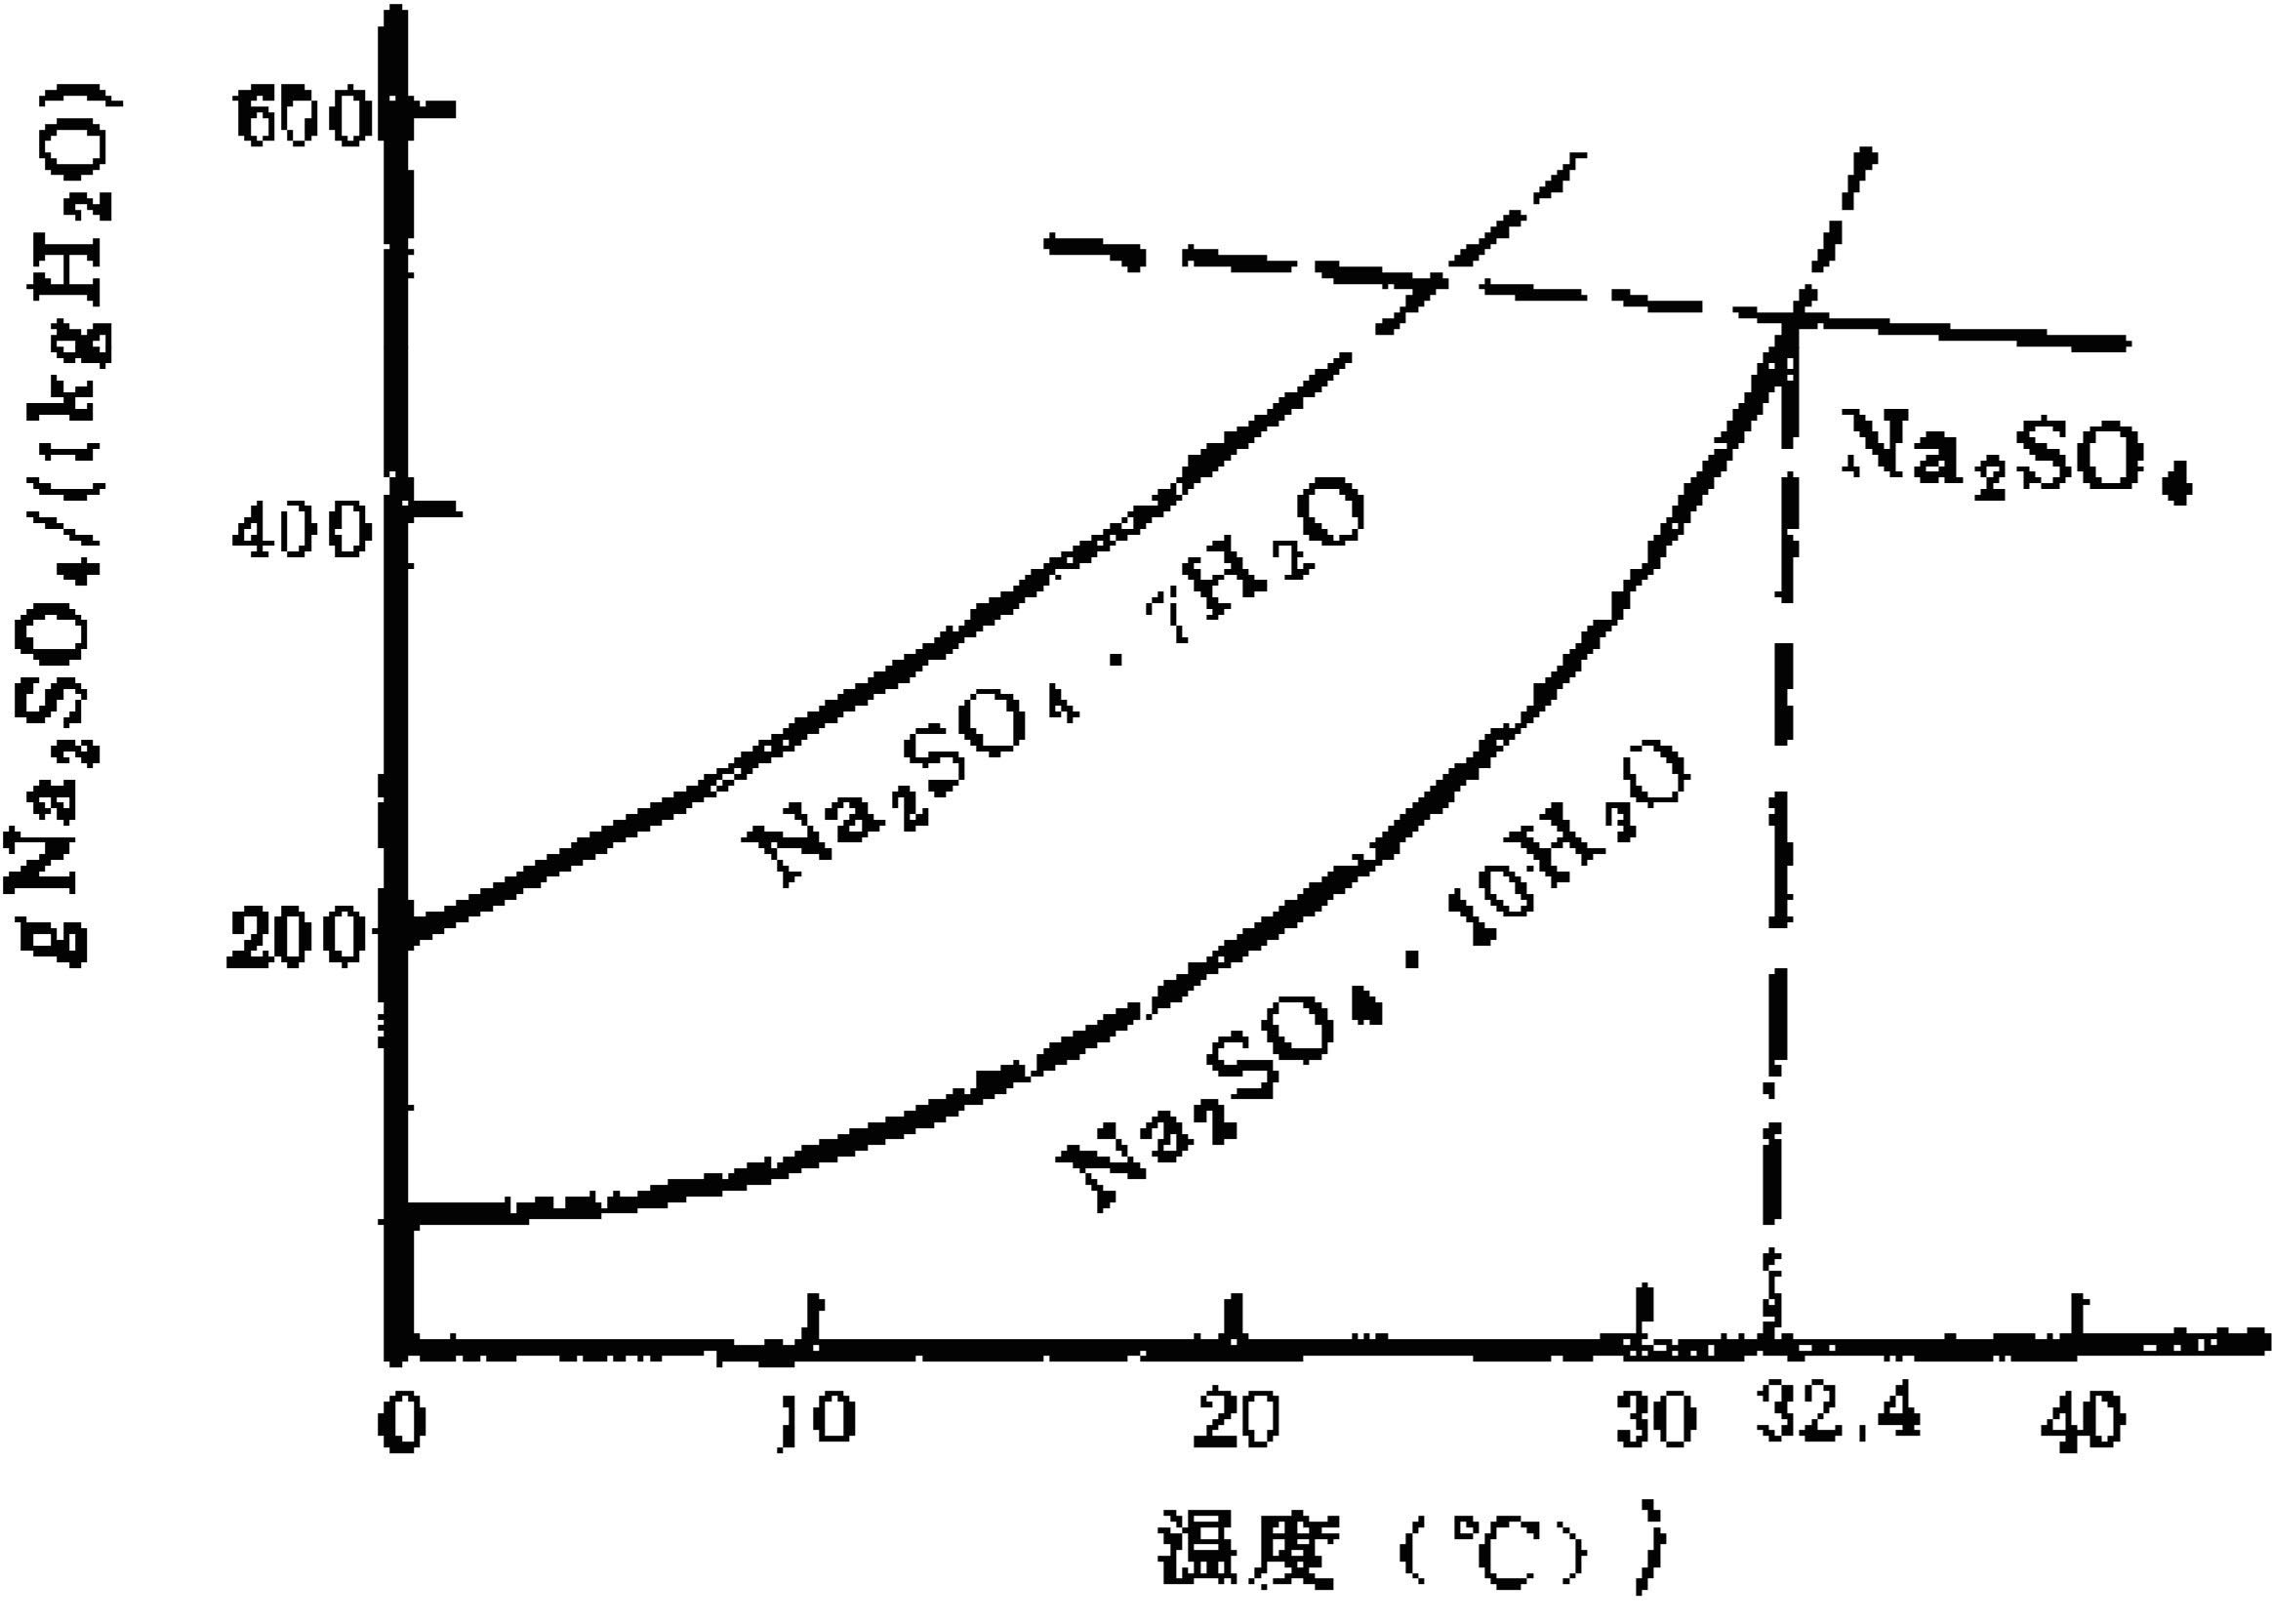
\includegraphics[width=0.8\textwidth]{fig/cp03/img3.14.jpg}
 \caption{$\rm Na_2SO_4-H_2O$体系。}
\end{figure}

\begin{figure}[h]
 \centering
 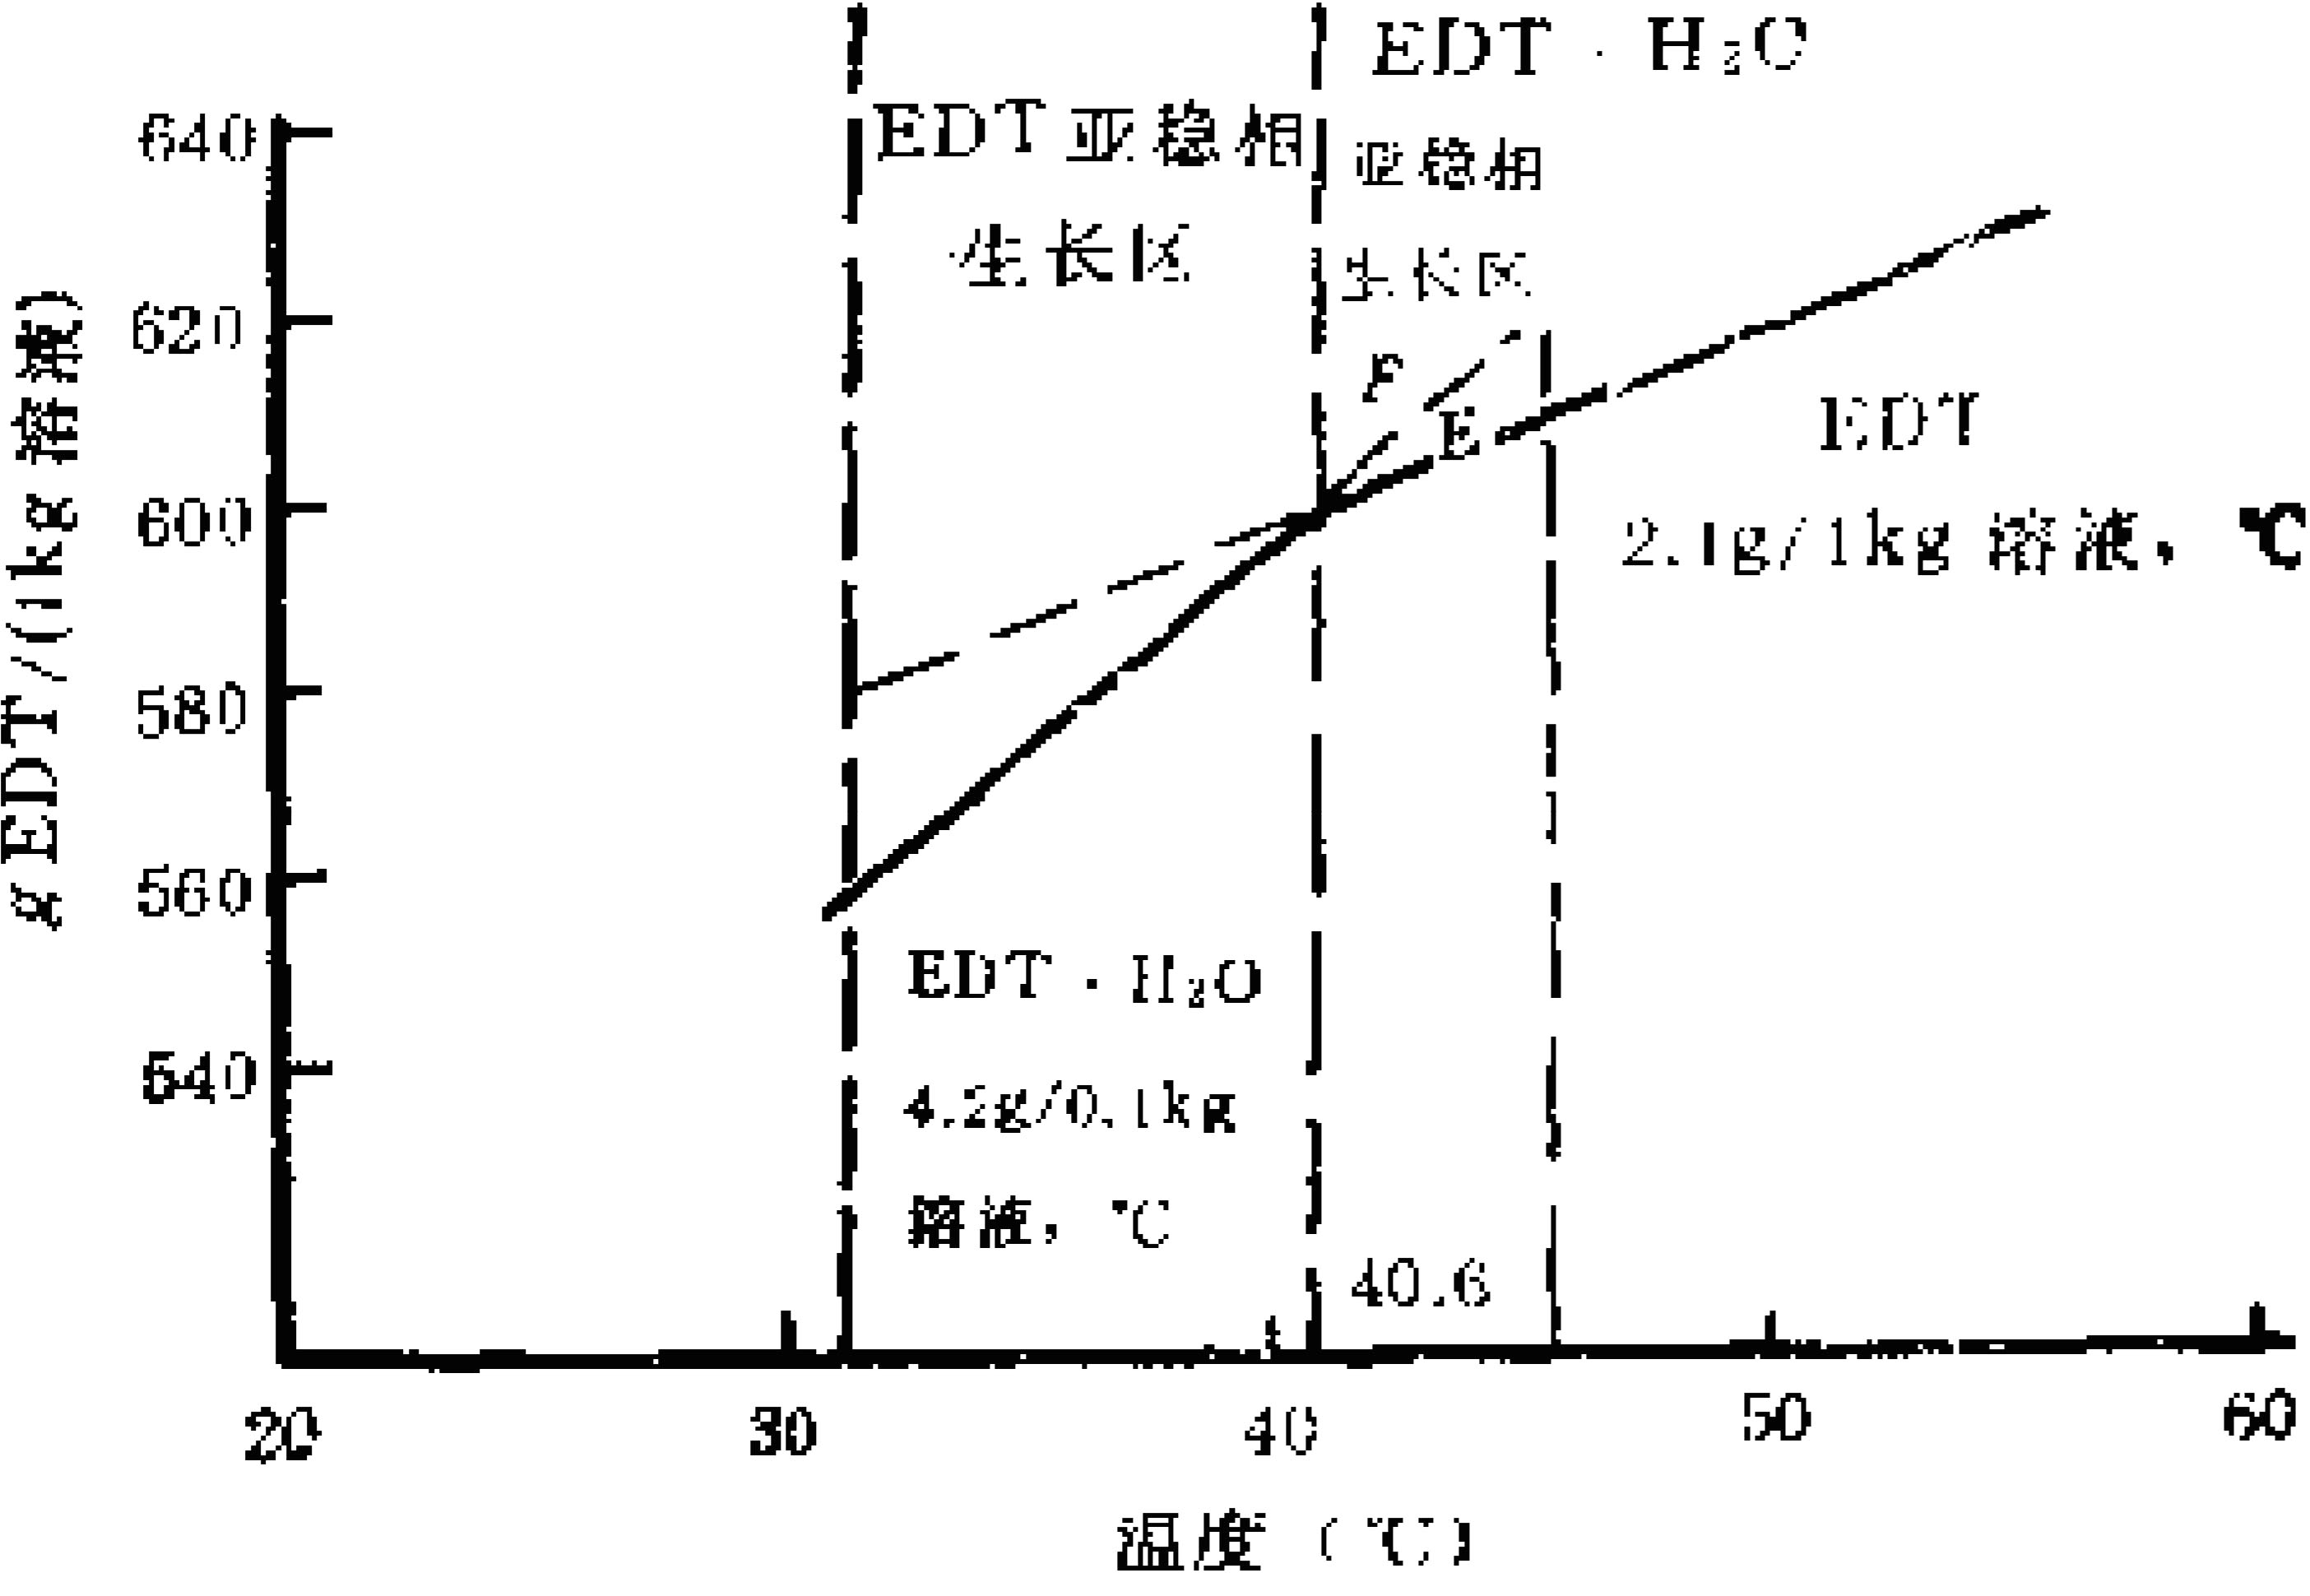
\includegraphics[width=0.8\textwidth]{fig/cp03/img3.15.jpg}
 \caption{$\rm EDT-H_2O$体系。}
\end{figure}

EDT在水溶液中,有EDT和$\rm EDT\cdot H_2O$两种结晶(图3.15)。这两个体系都是二组分体系,根据相律,在三相共存时只有一个自由度。如果压力固定(1atm),则体系是不变的。这就是说,两种晶相同时与溶液达成平衡的温度(即相平衡转变温度,以下简称转变温度)是完全确定的。硫酸钠的转变温度为32.4℃,EDT的转变温度为40.6℃。DKDP(通常为$\rm KD_{2x}H_{2(1-x)}PO_4$)在重水溶液中会出现四方和单斜两种结晶相,该体系可看成是$\rm DKDP-D_2O/D_2O+H_2O$准二组分体系,在三相达成平衡时,若压力固定(1atm),则两固相与溶液达成平衡的转变温度随$\rm DKDP-D_2O/D_2O+H_2O$的变化而变化。(图3.16)。对于D2O含量为99.8\%的溶液,DKDP的转变温度为21℃(见图3.11)

\begin{figure}[h]
 \centering
 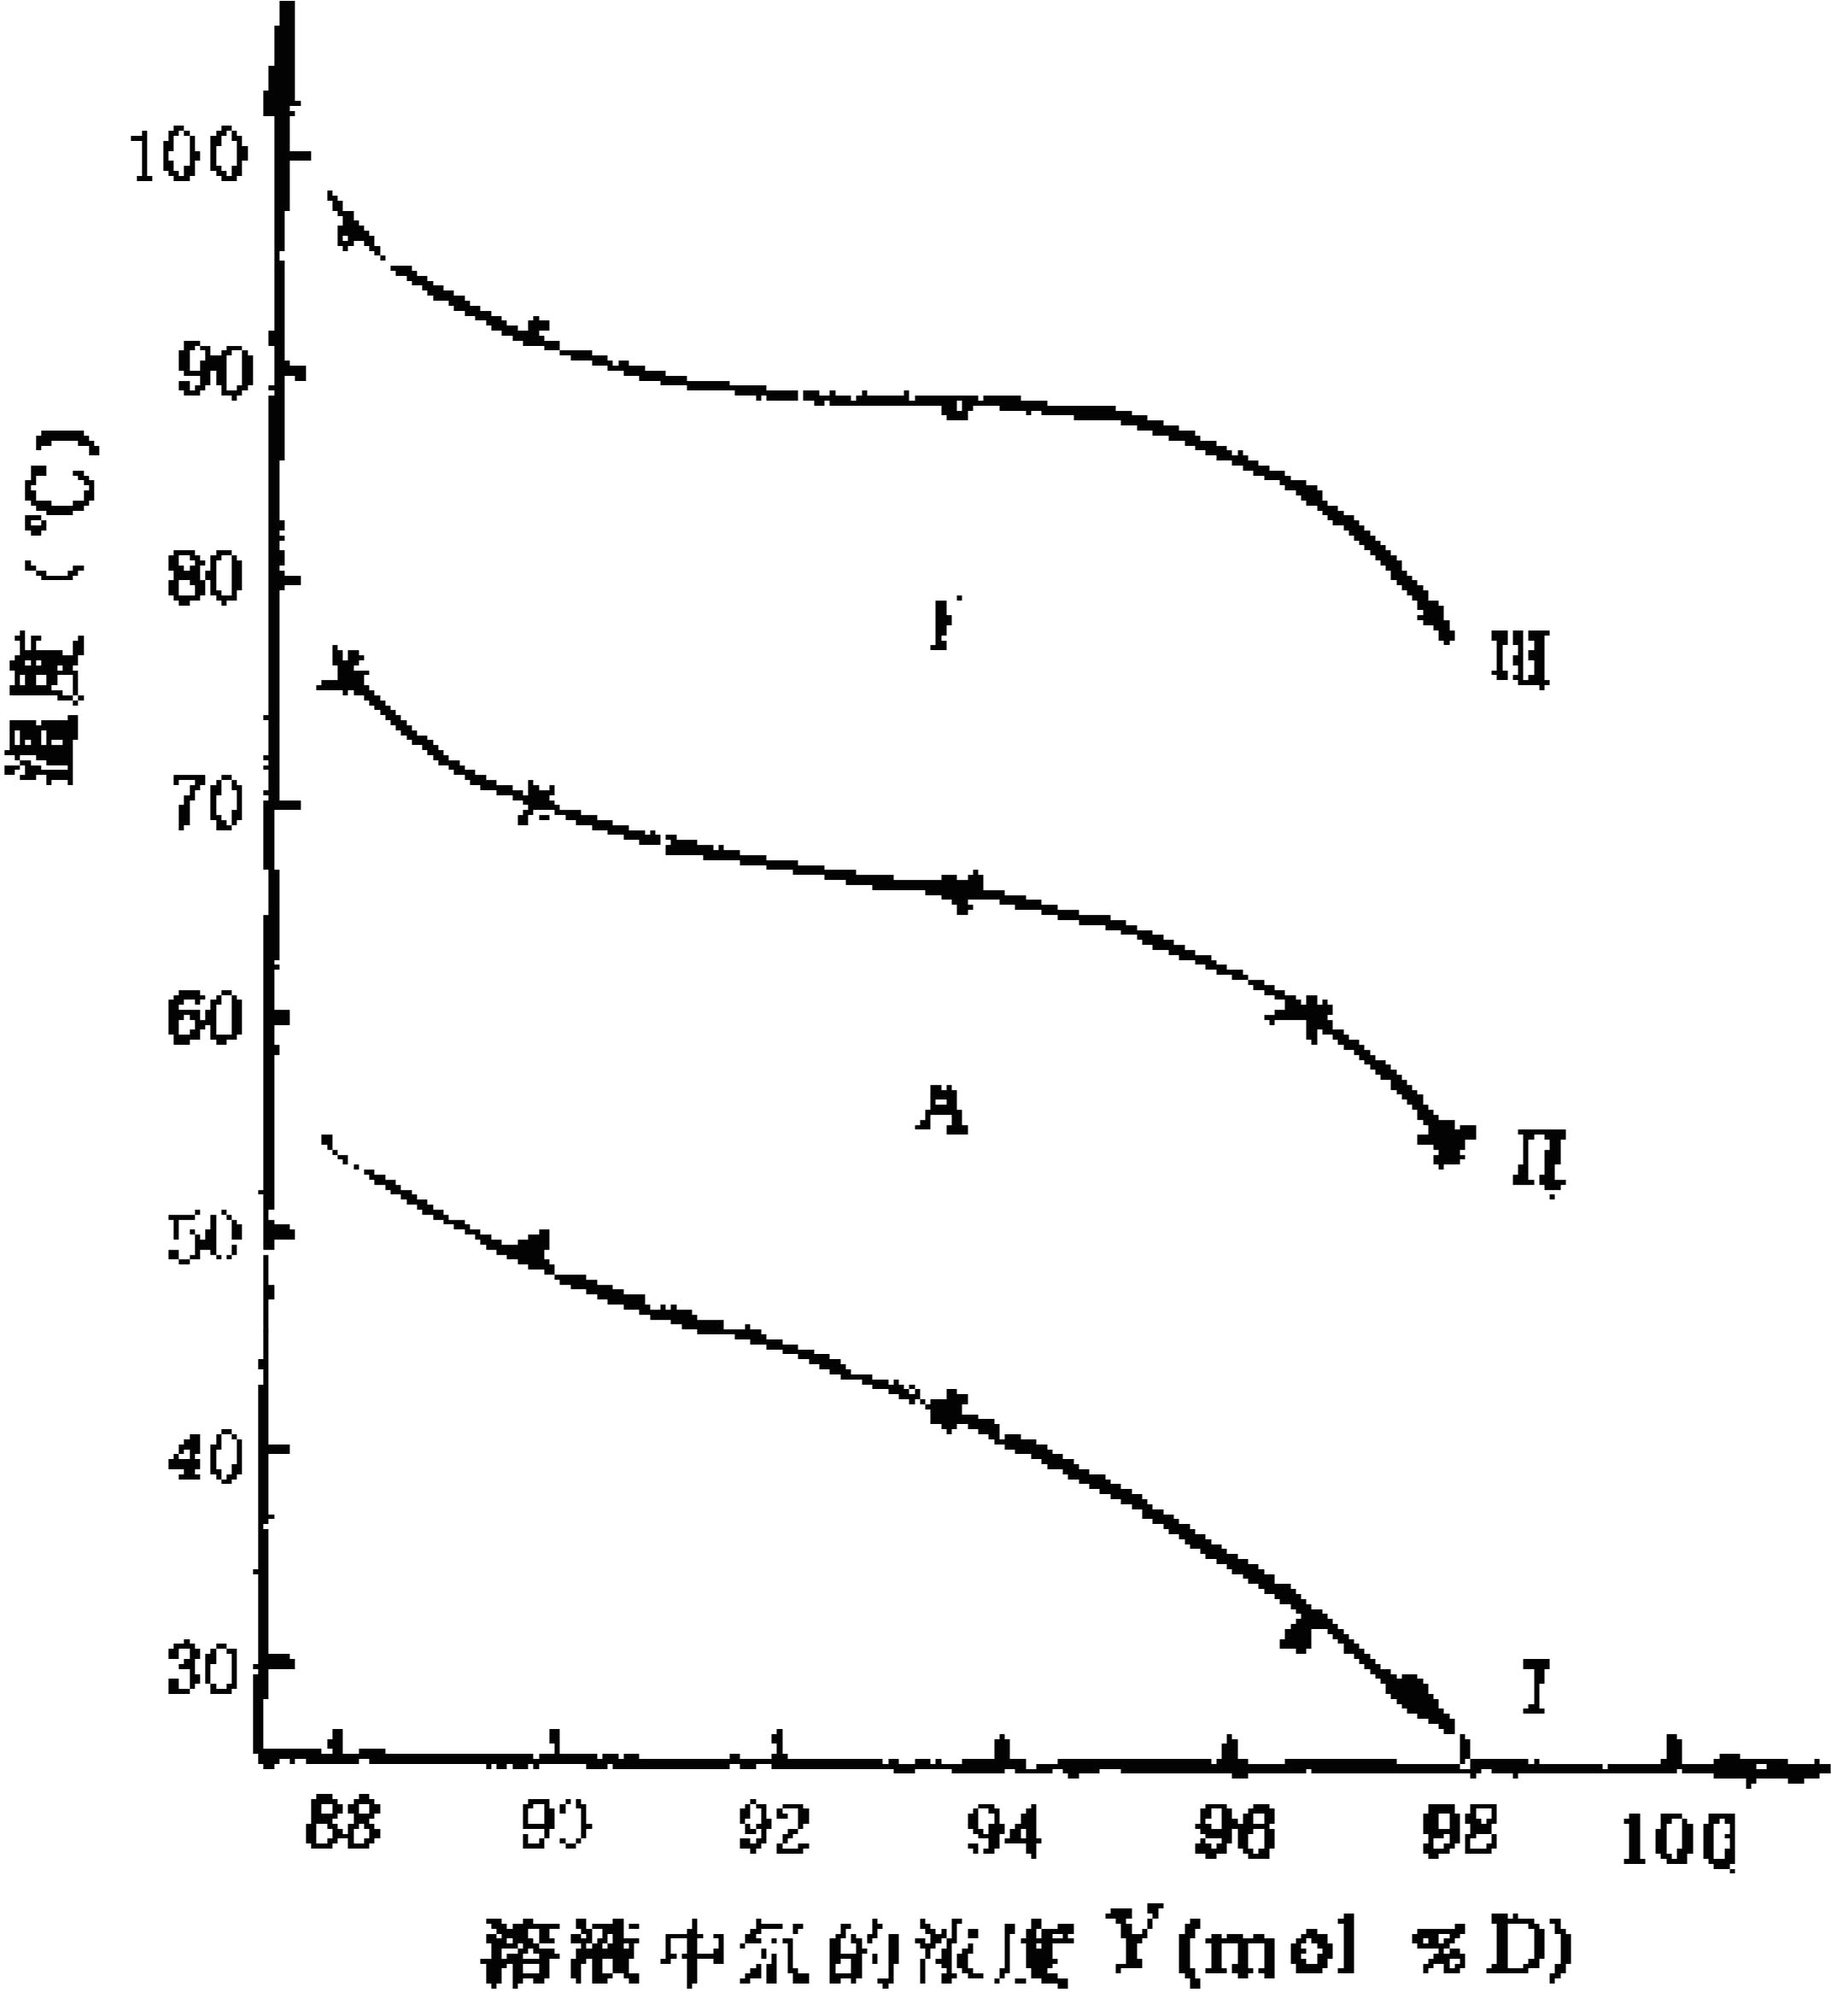
\includegraphics[width=0.8\textwidth]{fig/cp03/img3.16.jpg}
 \caption{四方和单斜DKDP的稳定区。}
\end{figure}

当溶液温度偏离转变点时,只能存在一种晶相与溶液平衡,另一种晶相将被溶解。但是晶体生长过程是一个不平衡的过程。如果溶液状态点处于两相溶解度曲线以上,如图3.15中的F点,则溶液对EDT无水物和水合物都是过饱和的,两相都可以生长,但无水物是稳定相,水合物是亚稳相,溶液相对于前者过饱和度较大,故生长速度也快。如果状态点在E,则EDT水合物生长,无水物溶解。但如果在无水物的稳定区内引入水合物籽晶,则水合物晶体即可在该区内实现亚稳相生长,长成$\rm EDT\cdot H_2O$大晶体,前提条件是溶液的过饱和度能满足$\rm EDT\cdot H_2O$晶体生长而又不致引起EDT稳定相自发成核。这是完全可能的,因为自发成核所需的过饱和度要比晶种上生长所需的过饱和度大得多。亚稳相生长区的界限可通过实验求出。不同物质和不同相的亚稳相生长区是不一样的。例如图3.14中,转变点以上,$\rm EDT\cdot H_2O$亚稳相生长区较窄(约6℃),而在转变点以下,EDT亚稳相生长区就较宽(约10℃)。对于DKDP,四方和单斜两相溶解度十分接近,亚稳相生长区比较宽,如对转变点为21℃的99.8\%的重水溶液,可以从43℃开始,用降温法成功地培养四方亚稳相晶体。图3.16粗略地示出在不同含氘量的重水溶液中,四方和单斜DKDP的亚稳相生长区。

溶液中的亚稳相晶体溶解度较大,在热力学上是不稳定的,它有自发地转变为溶解度较小的稳定相的趋势。例如,在离转变点较远的单斜稳定区中生长四方DKDP晶体时,在四方晶种上很容易长出单斜晶体,后者一旦出现即迅速生长,使四方母晶迅速被单斜晶体所“蚕食”。同样,在四方稳定区内生长单斜晶体时,也会出现四方晶体“蚕食”单斜母体的情况。

处于热力学不稳定状态的体系,在向其稳定状态过渡时,有时不是过渡到最稳定的状态(即自由能最低的状态),而是过渡到其自由能降低较小的中间状态。这一现象称为Ostwald阶段定律。例如在$\rm Na_2SO_4-H2O$体系中,有时从硫酸钠过饱和溶液中析出的不是稳定的$\rm Na_2SO_4\cdot 10H_2O$,而是亚稳相$\rm Na_2SO_4\cdot 7H_2O$(图3.14)。在DKDP的单斜稳定区中,有时也会析出亚稳的四方DKDP晶体(自发结晶实验证明,在图3.16上下两条虚线间析出的自发结晶既有单斜相,也有四方相),使溶液状态停留在亚稳四方相溶解度曲线附近,而不是直接降到单斜相溶解度曲线附近,虽然后者自由能降低更多,更为稳定。这样就有可能把溶液保持在中间状态,在这样的过饱和溶液中引入亚稳相籽晶,常常可以达到生长亚稳相晶体的目的。

在亚稳的条件下,生长亚稳相晶体有许多优点。许多高温变体如能在较低的温度下作为亚稳相自溶液中生长,则具有在本章开始时所述的优越性。在另一些情况下,由于某一相稳定区的局限性,需要在另一相的稳定区内生长。例如在氘化程度较高的重水溶液中,DKDP的转变温度很低,为了能在通常的温度区间用降温法生长出高含氘量的四方DKDP晶体,也可以在起始温度适当高于转变温度的情况下,使该晶体在单斜相稳定区内生长。图3.17示出的四方DKDP大晶体就是在这样的条件下生长出来的。在育晶器底部可以清楚地看见在生长过程中自发形成的单斜杂晶,由于溶液对这两相都是过饱和的,所以四方相和单斜相能同时存在和生长(但溶液和这两相并不处于平衡状态)。由此可见,亚稳相晶体生长的研究,在理论和实践上都是很有意义的。

\begin{figure}[h]
 \centering
 
\includegraphics[width=0.8\textwidth]{fig/cp03/img3.17.jpg}
 \caption{在单斜相稳定区内生长的DKDP大晶体($\rm 5.7\times 5.7\times 4.5cm$)}
\end{figure}

